\documentclass{memoria}


\begin{document}

\portada{Informe Entrega 3: Diseño Detallado}{Gerson Aguirre Pavez\\Max Chacón Villanueva\\Daniel Gacitúa Vásquez\\Elías González Marincovic\\Nicolás Rozas Sepúlveda}{\textbf{Profesores:}\\Mauricio Marín Caihuán\\Rodrigo Vásquez Fernández\\\textbf{Ayudante:\\}José Orellana}{\today}


\indices

\capitulonn{INTRODUCCIÓN.}



%-------------------------------------------------------------------------------------
\capitulo{MARCO TEÓRICO.}

\seccion{DIAGRAMA DE CASOS DE USO.}



\seccion{DIAGRAMAS DE SECUENCIA.}



%-------------------------------------------------------------------------------------
\capitulo{DIAGRAMA DE CLASES DE DISEÑO.}

\seccion{DIAGRAMA JAVAEE.}

\seccion{DIAGRAMA WEB-APP (ANGULAR JS).}

\seccion{DIAGRAMA LUCENE.}

\seccion{DIAGRAMA ANDROID.}
 

%-------------------------------------------------------------------------------------
\capitulo{CASOS DE USO.}

\seccion{CASO DE USO: REVISANDO HISTORIAL DE FOTOGRAFÍAS CARGADAS.} 

\tabla{Caso de Uso CU01}{
	\begin{tabular}[c]{|p{2.7cm}|p{13cm}|}
		\hline
		\textbf{ID}  & CU01\\ \hline
		\textbf{Nombre} & Revisando historial de fotografías cargadas\\ \hline
		\textbf{Resumen} & \\ \hline
		\textbf{Actores} & Usuario\\ \hline
		\textbf{Precondiciones} & \\ \hline
		\textbf{Descripción} & \\ \hline
		\textbf{Postcondiciones} & \\ \hline
		\textbf{Requisitos de Usabilidad} & \\ \hline
		\textbf{Excepciones} & \\ \hline
	\end{tabular}
}

\seccion{CASO DE USO: REVISANDO FOTOGRAFÍAS CARGADOS.}

\tabla{Caso de Uso CU02}{
	\begin{tabular}[c]{|p{2.7cm}|p{13cm}|}
		\hline
		\textbf{ID}  & CU02\\ \hline
		\textbf{Nombre} & Revisando fotografías cargadas\\ \hline
		\textbf{Resumen} & \\ \hline
		\textbf{Actores} & Usuario\\ \hline
		\textbf{Precondiciones} & \\ \hline
		\textbf{Descripción} & \\ \hline
		\textbf{Postcondiciones} & \\ \hline
		\textbf{Requisitos de Usabilidad} & \\ \hline
		\textbf{Excepciones} & \\ \hline
	\end{tabular}
}

\seccion{CASO DE USO: REVISANDO ÁLBUMES CREADOS.}

\tabla{Caso de Uso CU03}{
	\begin{tabular}[c]{|p{2.7cm}|p{13cm}|}
		\hline
		\textbf{ID}  & CU03\\ \hline
		\textbf{Nombre} & Revisando álbumes creados\\ \hline
		\textbf{Resumen} & \\ \hline
		\textbf{Actores} & Usuario\\ \hline
		\textbf{Precondiciones} & \\ \hline
		\textbf{Descripción} & \\ \hline
		\textbf{Postcondiciones} & \\ \hline
		\textbf{Requisitos de Usabilidad} & \\ \hline
		\textbf{Excepciones} & \\ \hline
	\end{tabular}
}

\seccion{CASO DE USO: VISUALIZANDO MAPA DE FOTOGRAFÍAS CARGADAS.}

\tabla{Caso de Uso CU04}{
	\begin{tabular}[c]{|p{2.7cm}|p{13cm}|}
		\hline
		\textbf{ID}  & CU04\\ \hline
		\textbf{Nombre} & Visualizando mapa de fotografías cargadas\\ \hline
		\textbf{Resumen} & \\ \hline
		\textbf{Actores} & Usuario\\ \hline
		\textbf{Precondiciones} & \\ \hline
		\textbf{Descripción} & \\ \hline
		\textbf{Postcondiciones} & \\ \hline
		\textbf{Requisitos de Usabilidad} & \\ \hline
		\textbf{Excepciones} & \\ \hline
	\end{tabular}
}

\seccion{CASO DE USO: EDITANDO LOCALIZACIÓN DE FOTOGRAFÍAS CARGADAS.}

\tabla{Caso de Uso CU05}{
	\begin{tabular}[c]{|p{2.7cm}|p{13cm}|}
		\hline
		\textbf{ID}  & CU05\\ \hline
		\textbf{Nombre} & Editanto localización de fotografías cargadas\\ \hline
		\textbf{Resumen} & \\ \hline
		\textbf{Actores} & Usuario\\ \hline
		\textbf{Precondiciones} & \\ \hline
		\textbf{Descripción} & \\ \hline
		\textbf{Postcondiciones} & \\ \hline
		\textbf{Requisitos de Usabilidad} & \\ \hline
		\textbf{Excepciones} & \\ \hline
	\end{tabular}
}

\seccion{CASO DE USO: VISUALIZANDO FOTOGRAFÍAS MARCADAS COMO FAVORITOS.}

\tabla{Caso de Uso CU06}{
	\begin{tabular}[c]{|p{2.7cm}|p{13cm}|}
		\hline
		\textbf{ID}  & CU06\\ \hline
		\textbf{Nombre} & Visualizando fotografías marcadas como favoritos\\ \hline
		\textbf{Resumen} & \\ \hline
		\textbf{Actores} & Usuario\\ \hline
		\textbf{Precondiciones} & \\ \hline
		\textbf{Descripción} & \\ \hline
		\textbf{Postcondiciones} & \\ \hline
		\textbf{Requisitos de Usabilidad} & \\ \hline
		\textbf{Excepciones} & \\ \hline
	\end{tabular}
}

\seccion{CASO DE USO: VISUALIZANDO ACTIVIDAD RECIENTE DE OTROS USUARIOS.}

\tabla{Caso de Uso CU07}{
	\begin{tabular}[c]{|p{2.7cm}|p{13cm}|}
		\hline
		\textbf{ID}  & CU07\\ \hline
		\textbf{Nombre} & Visualidando actividad reciente de otros usuarios\\ \hline
		\textbf{Resumen} & \\ \hline
		\textbf{Actores} & Usuario\\ \hline
		\textbf{Precondiciones} & \\ \hline
		\textbf{Descripción} & \\ \hline
		\textbf{Postcondiciones} & \\ \hline
		\textbf{Requisitos de Usabilidad} & \\ \hline
		\textbf{Excepciones} & \\ \hline
	\end{tabular}
}

\seccion{CASO DE USO: VISUALIZANDO FOTOGRAFÍAS DE USUARIOS A QUIENES SE ESTÁ SIGUIENDO.}

\tabla{Caso de Uso CU08}{
	\begin{tabular}[c]{|p{2.7cm}|p{13cm}|}
		\hline
		\textbf{ID}  & CU08\\ \hline
		\textbf{Nombre} & Visualizando fotografías de usuarios a quienes se está siguiendo.\\ \hline
		\textbf{Resumen} & \\ \hline
		\textbf{Actores} & Usuario\\ \hline
		\textbf{Precondiciones} & \\ \hline
		\textbf{Descripción} & \\ \hline
		\textbf{Postcondiciones} & \\ \hline
		\textbf{Requisitos de Usabilidad} & \\ \hline
		\textbf{Excepciones} & \\ \hline
	\end{tabular}
}

\seccion{CASO DE USO: VISUALIZANDO FOTOGRAFÍAS EN LAS QUE SE HAN MARCADO PERSONAS A LAS QUE SE ESTÁ SIGUIENDO.}

\tabla{Caso de Uso CU09}{
	\begin{tabular}[c]{|p{2.7cm}|p{13cm}|}
		\hline
		\textbf{ID}  & CU09\\ \hline
		\textbf{Nombre} & Visualizando fotografías en las que se han marcado personas a las que se está siguiendo\\ \hline
		\textbf{Resumen} & \\ \hline
		\textbf{Actores} & Usuario\\ \hline
		\textbf{Precondiciones} & \\ \hline
		\textbf{Descripción} & \\ \hline
		\textbf{Postcondiciones} & \\ \hline
		\textbf{Requisitos de Usabilidad} & \\ \hline
		\textbf{Excepciones} & \\ \hline
	\end{tabular}
}

\seccion{CASO DE USO: VISUALIZANDO FOTOGRAFÍAS RECIENTEMENTE CARGADAS A LA APLICACIÓN.}

\tabla{Caso de Uso CU10}{
	\begin{tabular}[c]{|p{2.7cm}|p{13cm}|}
		\hline
		\textbf{ID}  & CU10\\ \hline
		\textbf{Nombre} & Visualizando fotografías recientemente cargadas a la aplicación\\ \hline
		\textbf{Resumen} & \\ \hline
		\textbf{Actores} & Usuario\\ \hline
		\textbf{Precondiciones} & \\ \hline
		\textbf{Descripción} & \\ \hline
		\textbf{Postcondiciones} & \\ \hline
		\textbf{Requisitos de Usabilidad} & \\ \hline
		\textbf{Excepciones} & \\ \hline
	\end{tabular}
}

\seccion{CASO DE USO: VISUALIZANDO MAPA MUNDIAL DE FOTOGRAFÍAS CARGADAS.}

\tabla{Caso de Uso CU11}{
	\begin{tabular}[c]{|p{2.7cm}|p{13cm}|}
		\hline
		\textbf{ID}  & CU11\\ \hline
		\textbf{Nombre} & Visualizando mapa mundial de fotografías cargadas\\ \hline
		\textbf{Resumen} & \\ \hline
		\textbf{Actores} & Usuario\\ \hline
		\textbf{Precondiciones} & \\ \hline
		\textbf{Descripción} & \\ \hline
		\textbf{Postcondiciones} & \\ \hline
		\textbf{Requisitos de Usabilidad} & \\ \hline
		\textbf{Excepciones} & \\ \hline
	\end{tabular}
}

\seccion{CASO DE USO: VISUALIZANDO CÁMARAS QUE SE HAN UTILIZADO CON LA APLICACIÓN.}

\tabla{Caso de Uso CU12}{
	\begin{tabular}[c]{|p{2.7cm}|p{13cm}|}
		\hline
		\textbf{ID}  & CU12\\ \hline
		\textbf{Nombre} & Visualizando cámaras que se han utilizado con la aplicación\\ \hline
		\textbf{Resumen} & \\ \hline
		\textbf{Actores} & Usuario\\ \hline
		\textbf{Precondiciones} & \\ \hline
		\textbf{Descripción} & \\ \hline
		\textbf{Postcondiciones} & \\ \hline
		\textbf{Requisitos de Usabilidad} & \\ \hline
		\textbf{Excepciones} & \\ \hline
	\end{tabular}
}

\seccion{CASO DE USO: BUSCANDO PALABRAS CLAVE.}

\tabla{Caso de Uso CU13}{
	\begin{tabular}[c]{|p{2.7cm}|p{13cm}|}
		\hline
		\textbf{ID}  & CU13\\ \hline
		\textbf{Nombre} & Buscando palabra clave\\ \hline
		\textbf{Resumen} & \\ \hline
		\textbf{Actores} & Usuario\\ \hline
		\textbf{Precondiciones} & \\ \hline
		\textbf{Descripción} & \\ \hline
		\textbf{Postcondiciones} & \\ \hline
		\textbf{Requisitos de Usabilidad} & \\ \hline
		\textbf{Excepciones} & \\ \hline
	\end{tabular}
}

\seccion{CASO DE USO: SUBIENDO IMÁGENES.}

\tabla{Caso de Uso CU14}{
	\begin{tabular}[c]{|p{2.7cm}|p{13cm}|}
		\hline
		\textbf{ID}  & CU14\\ \hline
		\textbf{Nombre} & Subiendo imágenes\\ \hline
		\textbf{Resumen} & \\ \hline
		\textbf{Actores} & Usuario\\ \hline
		\textbf{Precondiciones} & \\ \hline
		\textbf{Descripción} & \\ \hline
		\textbf{Postcondiciones} & \\ \hline
		\textbf{Requisitos de Usabilidad} & \\ \hline
		\textbf{Excepciones} & \\ \hline
	\end{tabular}
}

\seccion{CASO DE USO: INTERACTUANDO CON FOTOGRAFÍAS CARGADAS.}

\tabla{Caso de Uso CU15}{
	\begin{tabular}[c]{|p{2.7cm}|p{13cm}|}
		\hline
		\textbf{ID}  & CU15\\ \hline
		\textbf{Nombre} & Interactuando con fotografías cargadas\\ \hline
		\textbf{Resumen} & \\ \hline
		\textbf{Actores} & Usuario\\ \hline
		\textbf{Precondiciones} & \\ \hline
		\textbf{Descripción} & \\ \hline
		\textbf{Postcondiciones} & \\ \hline
		\textbf{Requisitos de Usabilidad} & \\ \hline
		\textbf{Excepciones} & \\ \hline
	\end{tabular}
}


%-------------------------------------------------------------------------------------
\capitulo{DIAGRAMAS DE SECUENCIA.}


\seccion{DIAGRAMA DE SECUENCIA: REVISANDO HISTORIAL DE FOTOGRAFÍAS CARGADAS.} 

\seccion{DIAGRAMA DE SECUENCIA: REVISANDO FOTOGRAFÍAS CARGADOS.}

\seccion{DIAGRAMA DE SECUENCIA: REVISANDO ÁLBUMES CREADOS.}

\seccion{DIAGRAMA DE SECUENCIA: VISUALIZANDO MAPA DE FOTOGRAFÍAS CARGADAS.}

\seccion{DIAGRAMA DE SECUENCIA: EDITANDO LOCALIZACIÓN DE FOTOGRAFÍAS CARGADAS.}

\seccion{DIAGRAMA DE SECUENCIA: VISUALIZANDO FOTOGRAFÍAS MARCADAS COMO FAVORITOS.}

\seccion{DIAGRAMA DE SECUENCIA: VISUALIZANDO ACTIVIDAD RECIENTE DE OTROS USUARIOS.}

\seccion{DIAGRAMA DE SECUENCIA: VISUALIZANDO FOTOGRAFÍAS DE USUARIO A QUIENES SE ESTÁ SIGUIENDO.}

\seccion{DIAGRAMA DE SECUENCIA: VISUALIZANDO FOTOGRAFÍAS EN LAS QUE SE HAN MARCADO PERSONAS A LAS QUE SE ESTÁ SIGUIENDO.}

\seccion{DIAGRAMA DE SECUENCIA: VISUALIZANDO FOTOGRAFÍAS RECIENTEMENTE CARGADAS A LA APLICACIÓN.}

\seccion{DIAGRAMA DE SECUENCIA: VISUALIZANDO MAPA MUNDIAL DE FOTOGRAFÍAS CARGADAS.}

\seccion{DIAGRAMA DE SECUENCIA: VISUALIZANDO CÁMARAS QUE SE HAN UTILIZADO CON LA APLICACIÓN.}

\seccion{DIAGRAMA DE SECUENCIA: BUSCANDO PALABRAS CLAVE.}

\seccion{DIAGRAMA DE SECUENCIA: SUBIENDO IMÁGENES.}

\seccion{DIAGRAMA DE SECUENCIA: INTERACTUANDO CON FOTOGRAFÍAS CARGADAS.}


%-------------------------------------------------------------------------------------
\capitulo{DETALLE DE CASOS DE USO IMPLEMENTADOS.}

\seccion{CASO DE USO: REVISANDO FOTOGRAFÍAS CARGADAS.}

\seccion{CASO DE USO: REVISANDO ÁLBUMES CREADOS.}

%-------------------------------------------------------------------------------------
\capitulo{GESTIÓN DEL PROYECTO.}

\seccion{ORGANIZACIÓN DE REPOSITORIOS GIT.}
    
Para optimizar la creación de código, favorecer la correcta colaboración entre los integrantes y tener un versionamiento ordenado del código, se decide emplear a git como sistema de control de versiones, y usar GitHub como servidor remoto de git.\\

Cada miembro del grupo utiliza una cuenta de GitHub:

\begin{itemize}
	\item \textbf{Gerson Aguirre}: \textsl{https://github.com/GersonAguirre}
	\item \textbf{Max Chacón}: \textsl{https://github.com/nanochacon}
	\item \textbf{Daniel Gacitúa}: \textsl{https://github.com/GaciX}
	\item \textbf{Elías González}: \textsl{https://github.com/Elitos}
	\item \textbf{Nicolás Rozas}: \textsl{https://github.com/NicoRozas}
\end{itemize}

Se ha creado la organización “tbd2015” que aloja todos los repositorios del proyecto: \textsl{https://github.com/tbd2015}.\\

Dentro de la organización, se han creado diferentes repositorios para cada módulo del proyecto:

\begin{itemize}
	\item \textbf{InformesTBD}: Contiene los informes y presentaciones del proyecto. 
	\item \textbf{Prototipo}: Contiene el prototipo gráfico de la Aplicación Web.
	\item \textbf{BitPhoto}: Contiene el módulo principal del proyecto (en JavaEE).
	\item \textbf{BitPhoto-Mobile}: Contiene la aplicación para Android del proyecto.
	\item \textbf{BitPhoto-Search}: Contiene el motor de búsqueda (potenciado por Apache Lucene).
	\item \textbf{BitPhoto-Miner}: Contiene el módulo de análisis de sentimientos (potenciado por Weka).
	\item \textbf{BitPhoto-Web}: Contiene la aplicación web del proyecto (potenciado por Angular JS).
\end{itemize}

Cada miembro del grupo tendrá acceso a todos los repositorios para fomentar la colaboración. Cabe destacar que con un sistema modular de repositorios dentro de la organización ordena de mejor manera los aportes de cada miembro y ayuda a evitar el entorpecimiento al hacer commits de forma concurrente.

\newpage

\seccion{COMUNICACIÓN, AVANCES Y BURNDOWN.}

En la segunda reunión de planificación realizada, se determinó que el segundo\textsl{sprint} duraría hasta el 16 de Mayo del 2015. Además se acordó las horas de trabajo diarias que se podían dedicar a la realización del proyecto, se estimó que cada integrante del grupo podría dedicar a lo máximo 1.5 hrs al dia para el proyecto. Luego se definieron las tareas para que estas se pudieran realizar en un tiempo cercano al de trabajo diario estimado y posteriormente se estimó el tiempo que se demoraría cada tarea en estar realizada.

Para la realización de la segunda entrega el grupo optó por varios canales de comunicación para manejar las relaciones entre los participantes, por lo tanto se determinaron distintas tecnologías para objetivos específicos, los canales usados para comunicarse entre el grupo fueron los siguientes:


\begin{itemize}
	\item Grupo \textbf{\textsl{WhatsApp}}, con el fin de conversar inmediatamente y de forma rápida temas relacionados con el proyecto, principalmente se utilizó para dudas cortas y compartir pequeñas opiniones del proyecto.
	\item Grupo \textbf{\textsl{Facebook}}, para registrar minutas, información relevante y noticias que afecten a todos los integrantes del grupo.
	\item Se creo una carpeta en \textbf{\textsl{Google Drive}}, para con el fin de compartir documentos referentes al informe, presentaciones, entre otras, correspondientes a la entrega de diseño arquitectural.  
	\item Se utilizó la aplicación \textbf{\textsl{Trello}} para organizar las partes que se debían realizar en la entrega, además esta aplicación permite organizar las partes del proyecto definiendo las tareas personalmente y los tiempos con los que fueron realizadas cada una de estas.
	\item Para controlar las versiones del informe y los prototipo de las vistas se utilizó la herramienta \textbf{\textsl{Git}} que permite controlar las versiones de estas dos partes del proyecto. Esta tecnología se utiliza para archivos de texto plano y para controlar las modificaciones que se le pueden realizar a éstos.
\end{itemize}

\newpage

A continuación se presentan las tareas definidas y los tiempos estimados.

\figura{Tareas 1-21}{
	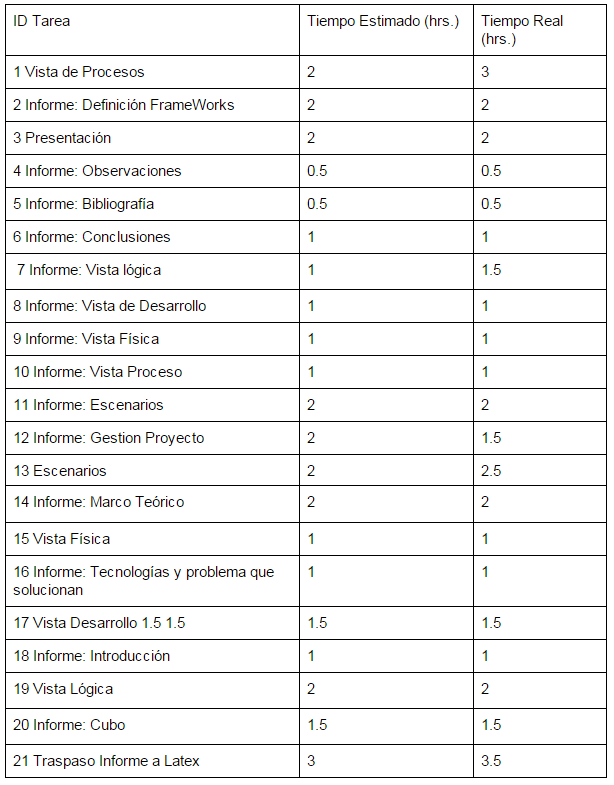
\includegraphics[width=15cm]{estimacionTareas1.png}
}


Ahora la cantidad de horas de trabajos estimadas son 31 hrs, Las horas de trabajo real fueron 33 hrs , notar que las horas reales trabajadas superaron las horas estimadas en 2 hrs aprox, esto quiere decir que las tareas se estimaron correctamente en su mayoría, ya que este margen de error fue relativamente bajo. Tiempo promedio por tarea fue de 1.48 hrs. Otros datos que se obtiene al analizar lo anterior son:

\begin{itemize}
	\item Estimación Trabajo Diario Grupo: 7.5 
	\item Horas Disponibles en Sprint por cada integrante: 37.5 
	\item Horas Disponibles en Sprint del Grupo: 187.5 
	\item Trabajo por dia promedio ideal 2.59 
\end{itemize}

Cabe señalar que si se trabajara de manera ideal, sobraría  tiempo equivalente a $187.5hrs - 31hrs = 156,5hrs$. 

A continuación se presentan los gráficos BurnDown y BurnUP con el fin de señalar la forma en que se trabajó a lo largo del Sprint.

\figura{Gráfico Burnup}{
	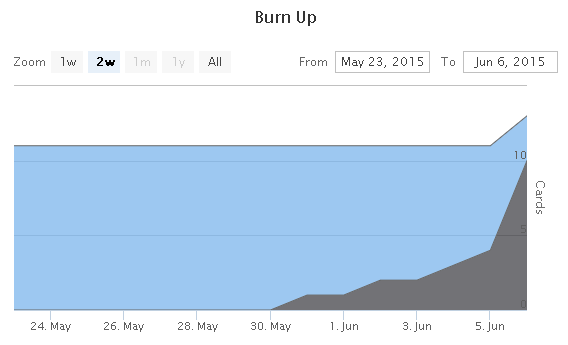
\includegraphics[width=15cm]{burnUp.png}
}

\newpage
\figura{Gráfico BurnDown}{
	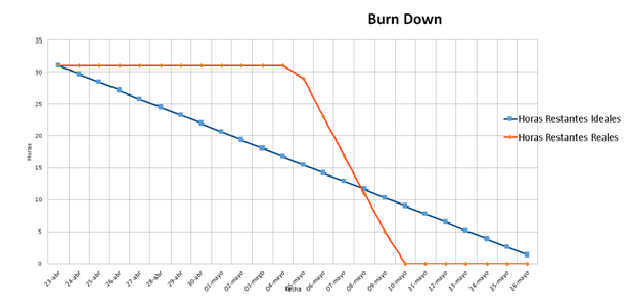
\includegraphics[width=15cm]{burnDown.png}
}

Como se aprecia en la imagen, se observa que en determinados periodos se trabajó una mayor cantidad, si bien alcanzamos a realizar la mitad del trabajo estimado a la fecha 8 de Mayo, se comenzó a trabajar en el proyecto varios días después de la planificación del \textsl{sprint}, por estos motivos se le solicitó al profesor mover la fecha de evaluación de la entrega de diseño arquitectural. Luego desde el 6 al 12 de mayo se comenzó a trabajar con gran rapidez, como se aprecia se terminó de ocupar las otras disponibles el 11 de mayo, el resto de los días si bien se trabajo, pero se trabajo tiempo superior al estimado.

Cabe destacar que para la próxima entrega se estimaron las tareas con \textsl{PokerPlaning} y se utilizará otra plataforma para realizar un análisis de datos, denominada \textsl{OllertApp}, la que facilitará el análisis de manera directa con lo realizado en \textsl{Trello}.

%-------------------------------------------------------------------------------------
\capitulo{OBSERVACIONES.}

Se añaden las observaciones realizadas al trabajo durante la 1º Presentación del Proyecto:

\tabla{Observación OBS1}{
	\begin{tabular}[c]{|p{4cm}|p{11cm}|}
		\hline
		Número Observación & OBS1\\ \hline
		Detalle Observación & Diagrama de Vista de Procesos mostrada en la presentación es en realidad Vista Física .\\ \hline
		Acción a Realizar & Diagrama mostrado se establece como Vista Física.\\ \hline
		Justificación & El diagrama mostrado permite representar de mejor manera la vista física que la de procesos.\\ \hline
		Página del Informe & 23\\ \hline
	\end{tabular}
}

\tabla{Observación OBS2}{
	\begin{tabular}[c]{|p{4cm}|p{11cm}|}
		\hline
		Número Observación & OBS2\\ \hline
		Detalle Observación & Eliminar servidor Android del diagrama de procesos mostrado (actualmente Vista Física).\\ \hline
		Acción a Realizar & Se elimina el servidor Android mostrado.\\ \hline
		Justificación & Servidor Android innecesario.\\ \hline
		Página del Informe & 23\\ \hline
	\end{tabular}
}

\tabla{Observación OBS3}{
	\begin{tabular}[c]{|p{4cm}|p{11cm}|}
		\hline
		Número Observación & OBS3\\ \hline
		Detalle Observación & Eliminar Managed Beans de los diagramas de secuencia de los Escenarios.\\ \hline
		Acción a Realizar & Se eliminan los Managed Beans de los diagramas de secuencia.\\ \hline
		Justificación & Innecesarios en el diagrama de secuencia, ya que no se utiliza Java Server Faces.\\ \hline
		Página del Informe & 31, 33 y 34\\ \hline
	\end{tabular}
}

\newpage

\tabla{Observación OBS4}{
	\begin{tabular}[c]{|p{4cm}|p{11cm}|}
		\hline
		Número Observación & OBS4\\ \hline
		Detalle Observación & Colocar Glassfish y JRE en la misma capa en diagrama 3-Dimensional SunTone.\\ \hline
		Acción a Realizar & Colocar Glassfish y JRE en la capa superior de los \textsl{Layers}.\\ \hline
		Justificación & Glassfish depende de JRE pero JRE no está por encima de Glassfish, por esto se colocan en la misma capa manteniendo JRE encima de Glassfish para representar la dependencia.\\ \hline
		Página del Informe & 35\\ \hline
	\end{tabular}
}

\tabla{Observación OBS5}{
	\begin{tabular}[c]{|p{4cm}|p{11cm}|}
		\hline
		Número Observación & OBS5\\ \hline
		Detalle Observación & Eliminar patrón DAO de la definición de \textsl{Frameworks}.\\ \hline
		Acción a Realizar & Eliminar DAO.\\ \hline
		Justificación & Patrón DAO no es un \textsl{Framework}, si bien viene implícito en JavaEE no se utiliza como tal.\\ \hline
		Página del Informe & 37\\ \hline
	\end{tabular}
}

%-------------------------------------------------------------------------------------
\capitulonn{CONCLUSIONES.}

Para la plataforma \textsl{BitPhoto}, es esencial diseñar correctamente el proyecto desde sus etapas más tempranas, es por eso que el Diseño Arquitectural es vital para el desarrollo y despliegue posterior de la aplicación.

El modelo 4+1 vistas y el Cubo 3D Suntone ayudan enormemente a llevar la visión de los arquitectos de software hacia los programadores, diseñadores y demás \textsl{stakeholders} de la aplicacion. En el contexto de la Ingeniería de Software resulta esencial comunicar correctamente la conceptualización de las ideas dentro del equipo de trabajo, para evitar inconsistencias en el producto final.

En esta entrega también se definen las tecnologías y sus versiones respectivas a utilizar dentro de la plataforma. Una clara definición del software y hardware que forman la plataforma condiciona la forma de trabajo, pero a la vez permite que los desarrolladores exploten de mejor manera los recursos tecnológicos disponibles.

Como siempre, la metodología ágil del proyecto implica constante comunicación entre los miembros del equipo desarrollador de \textsl{BitPhoto}. Llevando un control de las tareas desarrolladas se permite vigilar las cargas de trabajo.

Finalmente, se puede concluir que la plataforma \textsl{BitPhoto} pasó la etapa de Diseño Arquitectural, para iniciar posteriormente la etapa de Diseño Detallado. Los errores metodológicos a la hora de generar los esquemas y diagramas fueron debidamente corregidos.


%-------------------------------------------------------------------------------------

\capitulonn{BIBLIOGRAFÍA.}

[1] Philippe Kruchten. (Noviembre, 1995). En Planos Arquitectónicos: : El Modelo de “4+1” Vistas de la Arquitectura del Software(16). IEEE Software. 

Sitio Web: http://cic.puj.edu.co/wiki/lib/exe/fetch.php?media=materias:modelo4\_1.pdf

[2] SUNTONE ARCHITECTURE METHODOLOGY A 3-DIMENSIONAL APPROACH TO ARCHITECTURAL DESIGN. 11-Mayo-2015, de Sun MicroSystems 

Sitio web: http://rieck.dyndns.org/architecture/suntoneam\_wp\_5.24.pdf?version=1

[3] Chapter 2: Java Enterprise System Architecture. 11-Mayo-2015, de Sun Java Enterprise System 2004Q2 Technical Overview. 

Sitio web: https://docs.oracle.com/cd/E19263-01/817-5764/architecture.html

[4] Nicolás Tedeschi. ¿Qué es un Patrón de Diseño?. 11-Mayo-2015, de Microsoft 

Sitio web: https://msdn.microsoft.com/es-es/library/bb972240.aspx

[5] Juan Pavón Mestras. (2008-09). Estructura de las Aplicaciones Orientadas a Objetos El patrón Modelo-Vista-Controlador (MVC). 11-Mayo-2015, de Universidad Complutense Madrid 

Sitio web: https://www.fdi.ucm.es/profesor/jpavon/poo/2.14.MVC.pdf

[6] Libro J2EE Architecture \- B.V. Kumar, S. Sangeetha \& S.V. Subrahmanya [ISBN : 0070621632]

\end{document}
